\documentclass[letterpaper]{article}
\usepackage{graphicx}
\usepackage{amsfonts}
\usepackage{amsthm}
\usepackage{amsmath}
\usepackage{amssymb}
\usepackage{scribe}

% new packages used
\usepackage{mathpazo}
\usepackage{subcaption}

\usepackage[margin=1.5in]{geometry}
\linespread{1.1}
\graphicspath{{./fig/}}

% let's write a few macros to prevent carpal tunnel
\newcommand{\reals}{\mathbb{R}}
\providecommand\rbrac[1]{\ensuremath \left(#1\right)}
\providecommand\sqbrac[1]{\ensuremath \left[#1\right]}
\providecommand\cbrac[1]{\ensuremath \left\{#1\right\}}
\providecommand{\oor}{\vee}
\providecommand{\aand}{\wedge}
\providecommand{\bigo}{O}

\newcommand{\X}{X}
\newcommand{\Y}{Y}
\newcommand{\rk}{\mathrm{rk}}
\newcommand{\mf}{M_f}
\newcommand{\df}{D(f)}
\newcommand{\dnf}{D(\neg f)}
\newcommand{\nf}{N(f)}
\newcommand{\nnf}{N(\neg f)}
\newcommand{\cf}{C(f)}

% problems
\newcommand{\DISJ}{\mathrm{DISJ}}
\newcommand{\nDISJ}{\neg \mathrm{DISJ}}
\newcommand{\EQ}{\mathrm{EQ}}
\newcommand{\nEQ}{\neg \mathrm{EQ}}
\renewcommand{\P}{\mathrm{P}}
\newcommand{\NP}{\mathrm{NP}}
\newcommand{\coNP}{\mathrm{coNP}}

% hyperref
\usepackage[usenames,dvipsnames,svgnames,table]{xcolor}
\usepackage[bookmarks=true]{hyperref}
\hypersetup{
    colorlinks=true,
    linkcolor = violet,
    citecolor = brown,
    filecolor = magenta,
    urlcolor = blue
% use hidelinks option in hyperref to get black
}
\usepackage{url, cite}

\setlength{\marginparwidth}{1in}
\newcommand{\pc}[2]{{\color{brown} #1}\marginpar{\tiny\noindent{\raggedright{\color{ForestGreen}[PC]}\color{brown}{ #2} \par}}}
\newcommand{\todo}[1]{{\color{gray}#1}\marginpar{\tiny\noindent{\raggedright{\color{ForestGreen}[MILD TODO]}}}}


\begin{document}


\makeheader{Pratik Chaudhari}               % your name
           {October 20, 2014}               % lecture date
           {5}                              % lecture number
           {Log-rank conjecture and nondeterministic complexity}   % lecture title

\noindent

In this lecture, we first take a look at the log-rank conjecture. It has been conjectured that the deterministic communication complexity is essentially characterized by the log-rank of the characteristic matrix. In particular, it is at most the log-rank raised to a constant $c$. This is a major open problem and while the conjecture was first proposed with $c=1$, we will show here that $c$ in fact might be large.

We then introduce nondeterministic communication complexity where Alice and Bob are allowed to ``guess'' while executing the protocol. This is analogous the ``proof system'' approach, roughly speaking, Alice and Bob guess the smallest string that helps them to compute $f(x,y)$ without much communication. Just as we used partitions in the previous lectures to analyze deterministic complexity, we introduce covers of the characteristic matrix $\mf$; these effectively characterize the nondeterministic communication complexity of a function $f$.

Lastly, we compare and contrast the two notions of complexities. In particular, we show that the gap between deterministic and nondeterministic complexity can be exponentially large. This is surprising because we do not know whether such a result is true for the complexity classes $\P$ and $\NP$. However, we also show some functions $f$ where the nondeterministic complexity is almost as large as the deterministic complexity. We end the class after a brief discussion about the fact that nondeterministic and co-nondeterministic complexities cannot both be small.

\section{Log-rank conjecture}
\label{sec:log_rank}

We start the lecture with a discussion on the log-rank conjecture. We have already seen that log-rank of the characteristic matrix $\mf$ of a function $f : \X \times \Y \to \cbrac{0,1}$ is a very good lower bound on the deterministic communication complexity $\df$~\cite{mehlhorn1982vegas}. A prominent conjecture however is the following which states that $\df$ is essentially upper-bounded by the log-rank of $\mf$. This was first proposed by Lovasz and Saks~\cite{lovasz1988lattices} in a slightly different form.

\begin{conjecture}
\label{conj:log_rank}
For some constant $c > 0$, for all functions $f$,
$$
\log \rk (\mf) \leq \df \leq \sqbrac{\log \rk (\mf)}^c + c.
$$
\end{conjecture}
\begin{remark}
The original conjecture was proposed with $c=1$. However we will see today that $c$ is essentially large. In particular we shall prove that $\df \geq \sqbrac{\log \rk (\mf)}^{1.58}$.
Note that we have already proved the first inequality of the conjecture in previous classes, the second inequality on the other hand is a hard open problem in the field. To put things into perspective, we proved in the last lecture that
$$
\df \leq \rk_\reals (\mf) + 1
$$
which is an exponentially-worse upper bound than what the conjecture claims.
\end{remark}

Let us introduce the following theorem which quantifies the above discussion.
\begin{theorem}[Nisan and Wigderson~\cite{nisan1995rank}]
\label{thm:log_rank_bound}
There is a function $f: \cbrac{0,1}^n \times \cbrac{0,1}^n \to \cbrac{0,1}$ such that
$$
\df = \Omega(n) \qquad \mathrm{but},
$$
$$
\log \rk (\mf) \leq \bigo\rbrac{n^{\frac{1}{1.58\ldots}}}.
$$
\end{theorem}
\begin{remark}
First note that the above theorem implies $\df \geq \sqbrac{\log \rk (\mf)}^{1.58\ldots}$ which means that the constant $c$ in Conj.~\ref{conj:log_rank} is greater than $1.58$. To prove this theorem, we will construct a ``gadget'' and compose it with itself many times to construct a complicated function which will give us the above bounds.
\end{remark}
\begin{proof}
The basic idea of the proof is to construct a Boolean function with low degree and high ``sensitivity''. Define a real-valued polynomial with three binary inputs $h : \cbrac{0,1}^3 \to {0,1}$ as
$$
h(z_1, z_2, z_3) = z_1 + z_2 + z_3 - z_1 z_2 - z_2 z_3 - z_1 z_3.
$$
Note that $h$ is symmetric with respect to its arguments. We can now see that if exactly one of the $z$s is 1, $h = 1$, if exactly two $z$s are 1, we have $h = 1$. For all other cases, $h = 0$. In order words,
$$
h(z_1, z_2, z_3) = 
\begin{cases}
1 & \quad \mathrm{if}\ z_1 + z_2 + z_3 = 1\\
0 & \quad \mathrm{otherwise}.
\end{cases}
$$
Define a recursive function $H_d$ as shown in Fig.~\ref{fig:H_d}. To construct $H_d$, compose $h$ with itself $d$ times. In more cumbersome notation,
$$
H_d = h(H_{d-1}, H_{d-1}, H_{d-1}); \qquad H_0 = h.
$$
$H_d$ thus has $3^d$ leaves.

\begin{figure}
\centering
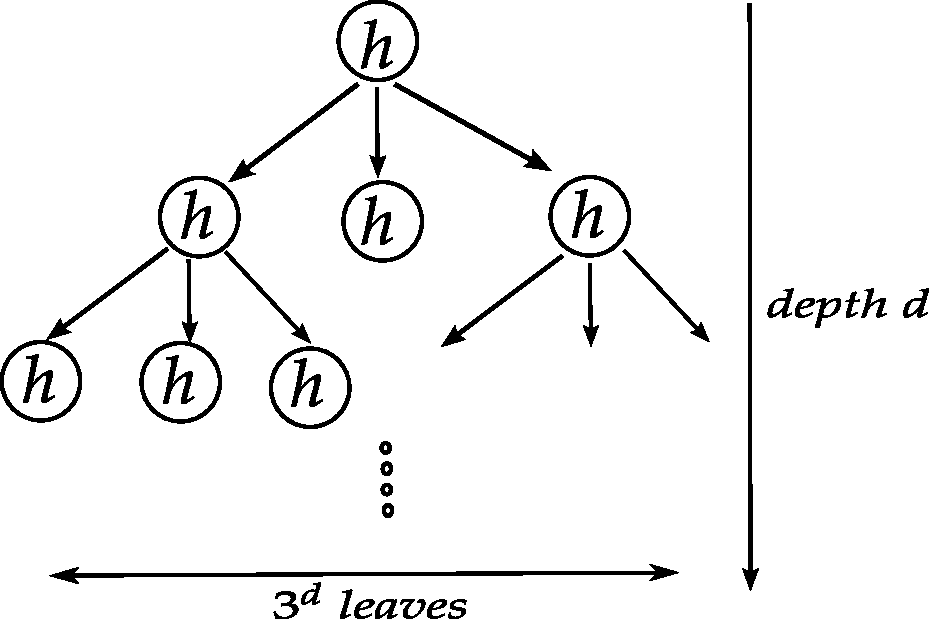
\includegraphics[width=0.5 \textwidth]{H_d.pdf}
\caption{$H_d$ is a function of $3^d$ inputs.}
\label{fig:H_d}
\end{figure}

We can also compute $H_d$ for a few special cases which we need, the others we do not care for.
$$
H_d(z_1, z_2, \ldots, z_{3^d}) =
\begin{cases}
1 & \quad \mathrm{if}\ \sum_{i} z_i = 1\\
0 & \quad \mathrm{if}\ \sum_{i} z_i = 0\\
\mathrm{don't\ care} & \quad \mathrm{otherwise}.
\end{cases}
$$
Let $f(x,y) = H_d(x \aand y)$, i.e., the length of the inputs of Alice and Bob, $n = 3^d$. Note that this is the set-disjointness problem, which is a prime example for a number of cornerstone results in communication complexity. We will see that the the rank lower bound implies that $\df \geq \Omega(3^d)$ for $f = H_d$.

To prove this theorem we will use a result which we have not proved yet, viz., for the disjointness problem $\DISJ_n$. This problem is really one of the cornerstones in the theory communication complexity and plays a large role in deriving important results. Well, in any case, we use the fact that $\df \geq \Omega(n) = \Omega(3^d)$ if $f = \DISJ_n$, proved by Razborov~\cite{razborov1992distributional}.

Why do we expect $\rk (\mf)$ to be low? Note that the degree of $h$ is 2, i.e., the degree of $H_d$ which is just $h$ composed $d$ times, is $2^d$. $h$ does not have full-degree, viz., 3.

\begin{proposition}
If $H_d = \sum_S c_S\ z_S$ where $z_S$ are monomials and $c_S$ are their coefficients ($S$ runs over all subsets of $\cbrac{1, \ldots, n}$), the rank $\rk (\mf)$ is at most the number of monomials $z_S$ that make up $H_d$, i.e.,
$$
\rk (\mf) \leq \mathrm{number\ of\ monomials\ in}\ H_d
$$
\end{proposition}
\begin{proof}
Note that
\begin{align*}
    \mf &= \sqbrac{H_d \rbrac{(x_1, y_1), \ldots, (x_n, y_n)}}\\
    &= \sum_k \sqbrac{\sum_S c_S M_S},
\end{align*}
where $M_S$ is the matrix defined by $M_S(x,y) = \prod_{i \in S}\ x_i \cdot y_i$. The entries of $M_S$ where $i \notin S$ or $j \notin S$ are zero. Now for every set $S$, the rank of $M_S$ is just 1. Using the rank inequalities, we can see that the rank $\rk \mf$ is bounded above by the number of non-zero monomials of $f$.
\end{proof}

\begin{proposition}
We also have 
$$
\mathrm{number\ of\ monomials\ in}\ H_d \leq 6^{2^d -1}.
$$
\end{proposition}
\begin{proof}
The proof of this proposition is a simple induction argument. Let $m_d$ be the number of monomials in $H_d$, note that $m_0 = 6$. In general,
$$
m_d \leq 3 m_{d-1} + 3 m_{d-1}^2; \qquad d = 1, 2, 3, \ldots
$$
Thus $m_d \leq 6 m_{d-1}^2$ which gives $m_d \leq 6^{2^d - 1}$.
\end{proof}

Together, the two propositions imply that
\begin{align*}
\df &\geq \Omega(3^d)\\
& \geq \Omega \rbrac{\sqbrac{\log \rk (\mf)}^{\log 3} }.
\end{align*}
\end{proof}

\begin{remark}
To repeat, the above theorem implies that $c > 1.58$. Let us note that $c$ can be improved slightly, using a gadget with 7 variables instead of 3. These gadgets are typically discovered using computer search and the one with 7 variables is the best result known to us yet.

A key takeaway from the development of this theorem is that rank bound is a very powerful method for computing the deterministic communication complexity. It works for all the problems that we (and other researchers elsewhere) have tried so far. The essential part of this program is however finding the right field to work in while computing the rank, most problems often become surprisingly easy when we use the right finite field.
\end{remark}


\section{Non-deterministic communication complexity}

Let us now introduce nondeterministic communication complexity. This was first discovered while analyzing the complexity of fabrication of large-scale digital circuits for various arithmetic tasks~\cite{lipton1981lower}. In the next few classes, we will explore the power of nondeterminism and contrast it with deterministic communication complexity. This model is analogous to the nondeterministic computational complexity and can be thought of as a ``proof system''. Roughly, nondeterministic communication complexity of a function $f$, denoted by $\nf$, is the smallest number of bits that can be used to convince both Alice and Bob that $f(x,y) = 1$. This is conceptually similar to $\mathrm{NP}$ languages, given the polynomial-length certificate, we can efficiently check if some input $x \in L \in \mathrm{NP}$.

\subsection{The model}

We know that deterministic protocols are binary trees. Each node of the tree is labeled either by a function $a_v : \X \to \cbrac{0,1}$ which corresponds to the bit sent by Alice or by a function $b_v : \Y \to \cbrac{0,1}$ which corresponds to Bob's bit. In addition to this, nondeterministic protocols have a special kind of node, a ``guess node'' which we will denote by $g_v \in \cbrac{0,1}$. At any point in the protocol execution, Alice and Bob can get together and ``publicly'' guess a value of $g_v \in \cbrac{0,1}$ upon which the protocol either moves left or right respectively in the protocol tree. An example nondeterministic protocol tree thus looks like the one shown in Fig.~\ref{fig:nondet_protocol_tree}. Note that while deterministic protocol trees have a unique path in the binary tree for a given pair of inputs $x, y$, the same is not true for nondeterministic protocols. Indeed, the power of nondeterminism lies in the fact that Alice and Bob and periodically guess together and branch.

\begin{figure}
\centering
\begin{subfigure}[b]{0.3 \textwidth}
    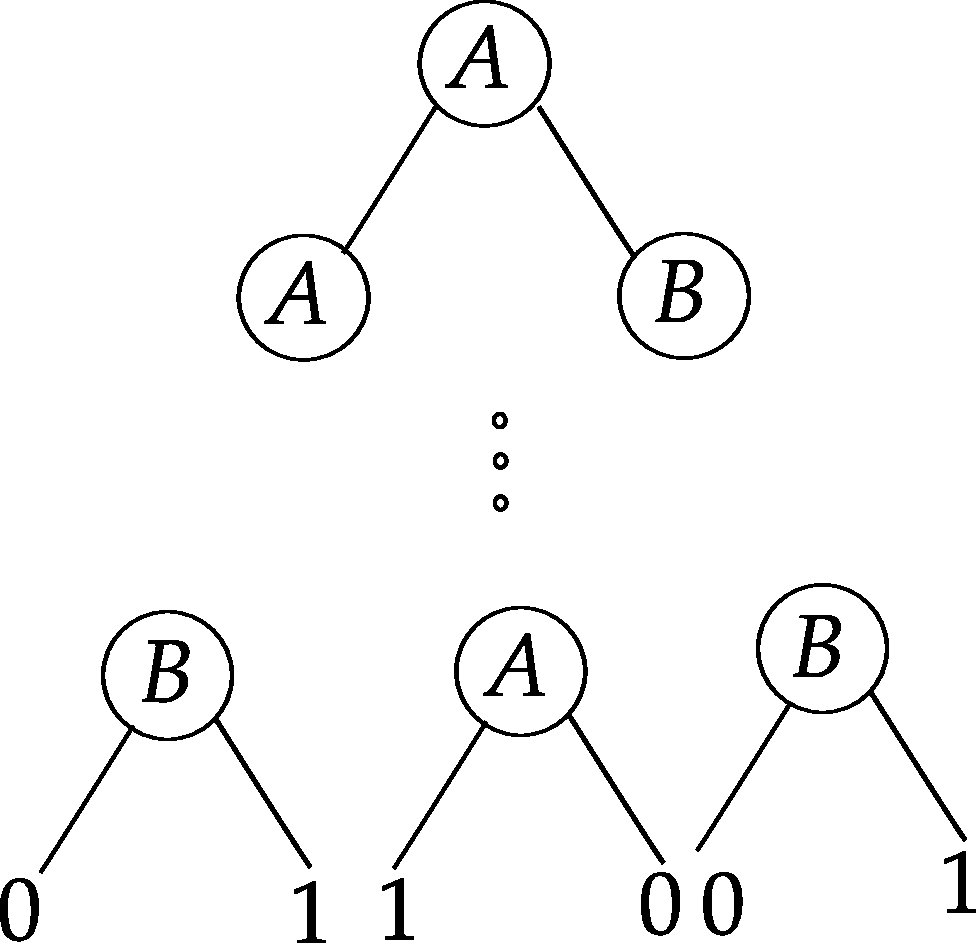
\includegraphics[width=\textwidth]{det_protocol.pdf}
    \caption{}
    \label{fig:det_protocol}
\end{subfigure}
\qquad \qquad
\begin{subfigure}[b]{0.3 \textwidth}
    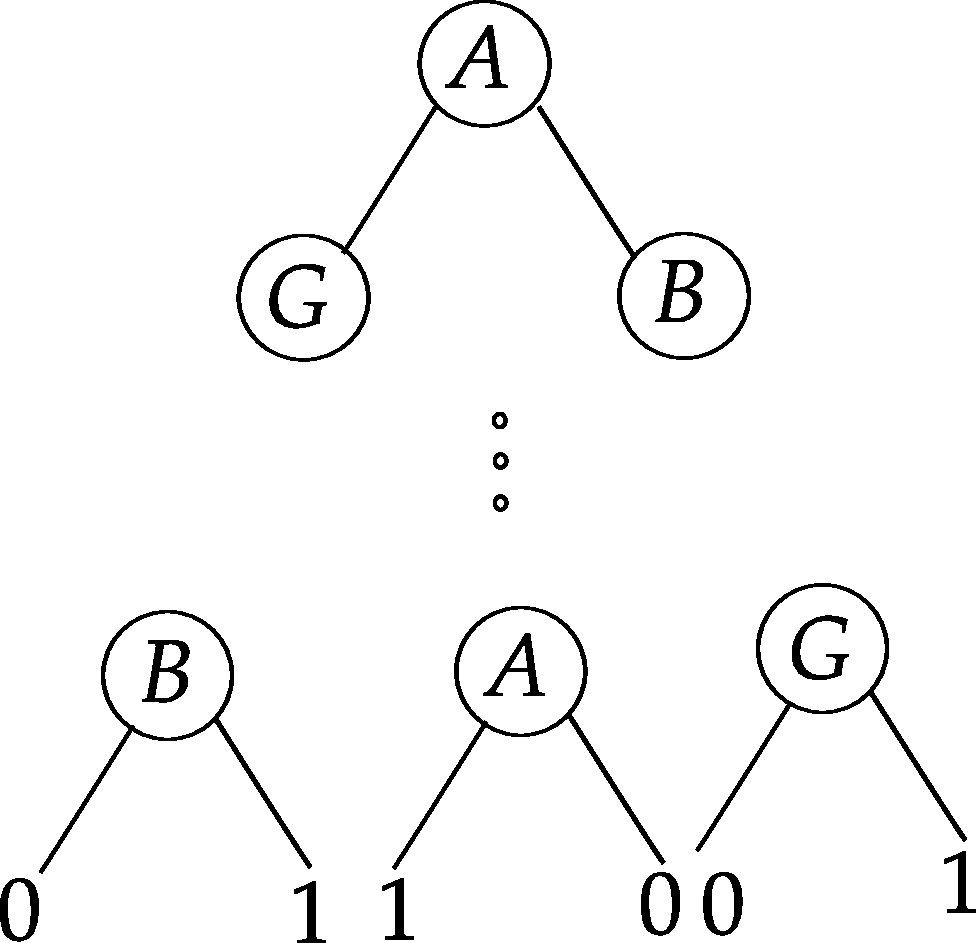
\includegraphics[width=\textwidth]{nondet_protocol.pdf}
    \caption{}
    \label{fig:nondet_protocol}
\end{subfigure}
\caption{Fig.~\ref{fig:det_protocol} shows a deterministic protocol. On the other hand, Fig.~\ref{fig:nondet_protocol} depicts the protocol tree for a nondeterministic protocol with guess nodes marked by $G$.}
\label{fig:nondet_protocol_tree}
\end{figure}

We have thus defined the syntax of a nondeterministic protocol tree. The semantics of this are as follows:
\begin{enumerate}
    \item at any point of time Alice or Bob can toss a coin to ``guess'' and outcome of this guess is public;
    \item coin tosses count towards communication cost;
    \item future messages depend upon previous messages as well as past coin-tosses;
    \item if $f(x, y) = 0$, the protocol must output a zero on \emph{all executions}, in other words, we do not tolerate any false positives;
    \item on the other hand, if $f(x, y) = 1$, the protocol only has to output one on at least one of the executions.
\end{enumerate}

\begin{definition}[Nondeterministic cost]
\label{def:nondet_cost}
The cost of a nondeterministic protocol is the worst case cost on any input and is equal to the sum of the number of bits exchanged and the number of coin tosses, i.e.,
$$
\nf = (\mathrm{\#\ of\ bits\ exchanged}) + (\mathrm{\#\ of\ coin\ tosses}).
$$
\end{definition}
\begin{remark}
Note that we are still following the usual definition for \emph{cost of a protocol}, it is simply the depth of the nondeterministic protocol tree. Also, note that coin tosses are costly, if we allow zero-cost coin tosses, any function $f$ will have a nondeterministic communication complexity of exactly $2$ bits. The following protocol achieves this --- Upon input $x, y$, Alice and Bob together guess some $x' \in \X$. Output $1$ if $x' = x$ and $f(x', y) = 1$ and zero otherwise. Note that Alice can check if $x' = x$, send the result to Bob who in turn computes the value of $f(x', y)$. This protocol has a cost of exactly 2 bits if Alice and Bob can guess $x'$ without any cost!
\end{remark}

\begin{proposition}
The nondeterministic communication complexity of any function $f : \X \times \Y \to \cbrac{0,1}$ is at most the deterministic communication complexity of $f$, i.e.,
$$
\nf \leq \df.
$$
\end{proposition}
\begin{proof}
Indeed, any deterministic protocol is also a nondeterministic protocol where Alice and Bob are happy with the general scheme of things and choose not to guess at all.
\end{proof}

Admittedly, the above discussion on nondeterministic protocols is rather abstract, let us discuss a few examples which will make the notion much more natural.

\begin{example}
The first example is the Inequality problem, denoted by $\nEQ_n$. Given two strings $x, y \in \cbrac{0,1}^n$, we need to check if $x \neq y$. The deterministic complexity of doing so is $n+1$ bits, Alice simply sends her input to Bob. Here is a nondeterministic protocol for the same problem.
\begin{enumerate}
    \item Guess an index $i \in \cbrac{1, \ldots, n}$;
    \item Output
         $$
            \begin{cases}
            1 & \mathrm{if}\ x_i \neq y_i\\
            0 & \mathrm{else.}
            \end{cases}
         $$
\end{enumerate}
First, let us compute the cost of this protocol. The first step costs $\log n$ bits while the second is just 2 bits. We thus have $N(\nEQ_n) = \log n + 2$. Why is this protocol a valid nondeterministic protocol? If $x \neq y$, there is at least one index on which they differ. Thus the protocol returns a one on at least one of the execution traces (precisely, the one where it guesses this index). If the two strings are equal, there does not exist any such index and the protocol returns zero. According to the ``proof system'' analogy, the certificate for two strings being unequal is simply the index on which they differ. Note that $D(\EQ_n) = D(\nEQ_n) = n+1$. How much is $N(\EQ_n)$? Stay tuned \ldots
\end{example}

\begin{example}
Let us discuss the problem of set intersection, denoted as $\nDISJ_n$. Given two subsets $A, B \subseteq \cbrac{1, \ldots, n}$, check if $A \cap B \neq \emptyset$. The nondeterministic protocol is as follows.
\begin{enumerate}
    \item Guess an element $i$;
    \item Output:
         $$
            \begin{cases}
            1 & \mathrm{if}\ i \in A \cap B\\
            0 & \mathrm{else.}
            \end{cases}
         $$
\end{enumerate}
Again, let us compute the cost of the protocol; it takes $\log n$ bits to guess an element $i$ and 2 bits for the second step of the protocol. Thus $N(\nDISJ_n) = \log n + 2$. It is instructive to verify if this is a valid nondeterministic protocol. It never gives false positives, if $A \cap B = \emptyset$, there does not exist any element $i$ that results in an output of 1 in the second step. The protocol always returns zero. Also, if $A \cap B \neq \emptyset$, a good certificate for this is simply the element that lies in both $A$ and $B$, our nondeterministic protocol guesses this element in $\log n$ bits.
\end{example}

\subsection{Nondeterminism and covers}

In the deterministic case, we saw that the log-rank effectively characterizes the communication complexity. In the nondeterministic case, we will see that the analogous concept is a ``cover''. Covers are more convenient combinatorial objects than partitions and the relation between covers and nondeterminism is very natural. Before we introduce notation, Fig.~\ref{fig:cover_example} shows an example cover. All the 1s in the matrix shown in Fig.~\ref{fig:cover_example} can be covered by 2 monochromatic rectangles.
\begin{figure}
\centering
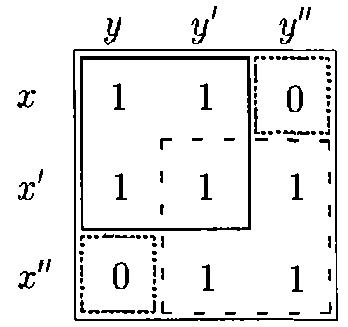
\includegraphics[width=0.3 \textwidth]{cover_example}
\caption{An example cover for the characteristic matrix. The cover number $\cf$ is therefore 2.}
\label{fig:cover_example}
\end{figure}

\begin{definition}[Cover number]
The cover number of a function $f : \X \times \Y \to \cbrac{0,1}$, denoted by $\cf$ is the minimum number of $f$-monochromatic rectangles $R_1, R_2, \ldots$ required to cover all the 1s in the characteristic matrix $\mf$, i.e.,
$$
\cup R_i = f^{-1}(1).
$$
\end{definition}
Note that $R_i$s in the above definition may overlap, we simply require that their union be $f^{-1}(1)$. The following theorem now effectively characterizes the nondeterministic communication complexity in terms of the cover number.

Note that we have not explicitly stated the notion of a rectangle for nondeterministic protocols. There are two ways to see this and they are equivalent. One can simply consider the characteristic matrix $\mf$ and an $f$-monochromatic rectangle $R$ is a set which can be written as a product of two sets $R_X \times R_Y$ where $R_X = \cbrac{ x\ |\ \exists\ y\ \mathrm{s.t.}\ (x,y) \in R}$ and $R_Y = \cbrac{ y\ |\ \exists\ x\ \mathrm{s.t.}\ (x,y) \in R}$. Alternatively, consider two input pairs $(x,y)$ and $(x', y')$. Let the guesses for Alice and Bob for these two pairs be $(z_1, z_2)$ for input $(x,y)$ and $(z_1', z_2')$ for input $(x',y')$ respectively. \pc{If $(x,y), (x',y') \in f^{-1}(1)$, there exist}{}

\begin{theorem}
For all functions $f$,
$$
\log \cf \leq \nf \leq \log \cf + 3.
$$
\end{theorem}
\begin{proof}
Let us prove the second inequality first. If $c = \cf$, let $R_1, \ldots, R_c$ be a cover for 1s in $\mf$. Here is a protocol for computing $f$.
\begin{enumerate}
    \item Guess the index of rectangle $i$;
    \item Output
        $$
            \begin{cases}
            1 & \mathrm{if}\ (x,y) \in R_i;\\
            0 & \mathrm{else.}
            \end{cases}
         $$
\end{enumerate}
Note that it takes $\lceil \log c \rceil$ bits to guess an index and 2 bits for the second step. In total, $\nf \leq \log c + 3$.

The first inequality can be proved in a similar way as the deterministic communication complexity version. Fix a nondeterministic protocol for $f$ with cost $\nf$. Let
$$
R_l = \cbrac{ (x,y)\ \mathrm{such\ that\ leaf}\ l\ \mathrm{is\ reachable\ on\ input}\ (x,y) }.
$$

\end{proof}


\subsection{Deterministic vs. Nondeterministic complexity}

Let us introduce some relationships between deterministic and nondeterministic complexities. The results here are quite surprising when contrasted with similar conjectures in computational complexity. Indeed, as far as communication complexity is concerned, the gap between deterministic and nondeterministic complexities is exponentially large. Moreover, we also know examples where the gap is precisely that big.

\begin{theorem}
\label{thm:det_vs_nondet}
For all functions $f$,
$$
\nf \leq \df \leq 2^{\nf} + 1.
$$
\end{theorem}
\begin{proof}
The first inequality is trivial and we have seen it before. The second inequality is striking. Let us prove it below. As usual, let $c = \cf$ and let $R_1, \ldots, R_c$ be rectangles that form a 1-cover. Here is a deterministic protocol for computing $f(x,y)$.
\begin{enumerate}
    \item Alice sends Bob, $b_1, \ldots, b_c$ where each $b_i$ is 1 if $x \in R_i$ and zero otherwise.
    \item Bob outputs
        $$
            \begin{cases}
            1 & \mathrm{if}\ y \in R_l\ \mathrm{and}\ b_l = 1;\\
            0 & \mathrm{else.}
            \end{cases}
         $$
\end{enumerate}
It is clear that the cost of this protocol is $c$ bits for step 1 and 1 bit for step 2, i.e.,
$$
\df \leq c+1 \leq 2^{\nf} + 1.
$$
\end{proof}

\begin{remark}
Thm.~\ref{thm:det_vs_nondet} is tight on both inequalities. We have shown before that $D(\nEQ_n) = n+1$, Alice simply sends her entire input. On the other hand, the nondeterministic complexity of this is $C(\nEQ_n) = \lceil \log n \rceil + 2$, we guess the index of the errant element in the two strings. This shows that
$$
D(f) \geq \Omega \rbrac{2^\nf}; \qquad f = \nEQ_n.
$$
On the other hand, consider $f = \EQ_n$, for which we know that $\df = n+1$. It can be shown using the fooling set method that certificate for $\EQ_n$ is at least $2^n$ bits long, which implies $\nf \geq n$.
\end{remark}

Observe that $\df = \dnf$, Alice and Bob simply output the opposite of what they would have given for $(x,y)$ after executing the protocol. However, $\nf$ and $\nnf$ are vastly different. While the gap between $\df$ and $\nf$ can be exponential as shown in Thm.~\ref{thm:det_vs_nondet}, we have the following remarkable result that
$$
\df \leq 2 \nf \nnf.
$$
We will prove this in the next lecture. $\nnf$ is the co-nondeterministic communication complexity. This result thus says that either the nondeterministic or co-nondeterministic complexity of a function $f$ can be small, but not both. (Stretching the analogy with complexity theory even further) contrast this with the open problem that asks whether $\P = \NP \cap \coNP$~\cite{papadimitriou1984communication}. In the other direction, if $f$ has nondeterministic and co-nondeterministic complexity of $t$, the deterministic complexity can be at most $\bigo(t^2)$.


\bibliographystyle{abbrv}
\bibliography{lec5}

\end{document}
